
\let\negmedspace\undefined
\let\negthickspace\undefined
\documentclass[journal]{IEEEtran}
\usepackage[a5paper, margin=10mm, onecolumn]{geometry}
%\usepackage{lmodern} % Ensure lmodern is loaded for pdflatex
\usepackage{tfrupee} % Include tfrupee package

\setlength{\headheight}{1cm} % Set the height of the header box
\setlength{\headsep}{0mm}     % Set the distance between the header box and the top of the text

\usepackage{gvv-book}
\usepackage{gvv}
\usepackage{cite}
\usepackage{amsmath,amssymb,amsfonts,amsthm}
\usepackage{amsmath}
\usepackage{algorithmic}
\usepackage{graphicx}
\usepackage{textcomp}
\usepackage{xcolor}
\usepackage{txfonts}
\usepackage{listings}
\usepackage{enumitem}
\usepackage{mathtools}
\usepackage{gensymb}
\usepackage{comment}
\usepackage[breaklinks=true]{hyperref}
\usepackage{tkz-euclide} 
\usepackage{listings}
% \usepackage{gvv}                                        
\def\inputGnumericTable{}                                 
\usepackage[latin1]{inputenc}                                
\usepackage{color}                                            
\usepackage{array}                                            
\usepackage{longtable}                                       
\usepackage{calc}                                             
\usepackage{multirow}                                         
\usepackage{hhline}                                           
\usepackage{ifthen}                                           
\usepackage{lscape}
\usepackage{circuitikz}
\tikzstyle{block} = [rectangle, draw, fill=blue!20, 
    text width=4em, text centered, rounded corners, minimum height=3em]
\tikzstyle{sum} = [draw, fill=blue!10, circle, minimum size=1cm, node distance=1.5cm]
\tikzstyle{input} = [coordinate]
\tikzstyle{output} = [coordinate]


\begin{document}

\bibliographystyle{IEEEtran}
\vspace{3cm}

\title{8.2.56}
\author{AI25BTECH11018-Hemanth Reddy}
 \maketitle
% \newpage
% \bigskip
{\let\newpage\relax\maketitle}

\renewcommand{\thefigure}{\theenumi}
\renewcommand{\thetable}{\theenumi}
\setlength{\intextsep}{10pt} % Space between text and floats


\numberwithin{equation}{enumi}
\numberwithin{figure}{enumi}
\renewcommand{\thetable}{\theenumi}

\textbf{Question:}\\

Given the ellipse with equation $9x^{2} + 25y^{2} = 225$, find the eccentricity and foci.
\textbf{Solution:}\\






Step 1: Represent the Ellipse in Matrix Form\\
\begin{align}
   \text{ The given equation of the ellipse is }9x^2 + 25y^2 = 225
\end{align}

\begin{align}
     \text{  The general form of conic is} \quad g(\vec{x}) = \vec{x}^{\text{T}} \vec{V} \vec{x} + 2\vec{u}^{\text{T}} \vec{x} + f = 0
\end{align}
By rearranging the terms:
\begin{align}
    9x^2 + 25y^2 - 225 = 0
\end{align}

By comparing the equation to the general form, we identify the matrices and vectors:
\begin{align}
    \vec{x} = \myvec{ x \\ y }, \quad \vec{V} = \myvec{ 9 & 0 \\ 0 & 25 }, \quad \vec{u} = \myvec{ 0 \\ 0 }, \quad f = -225
\end{align}


Step 2: Find the Eccentricity\\


The eccentricity $e$ is given by the formula $e = \sqrt{1 - \frac{\lambda_1}{\lambda_2}}$, where $\lambda_1$ and $\lambda_2$ are the eigenvalues of the matrix $\vec{V}$. For our diagonal matrix $\vec{V}$, the eigenvalues are the diagonal entries:
$
\lambda_1 = 9 \quad \text{and} \quad \lambda_2 = 25
$\\
\begin{align}
    \text{Using the formula:}
e = \sqrt{1 - \frac{9}{25}} = \sqrt{\frac{25-9}{25}} = \sqrt{\frac{16}{25}} = \frac{4}{5}
\end{align}


The eccentricity of the ellipse is $\frac{4}{5}$.

Step 3: Find the Foci\\



The foci lie on the major axis, and their location depends on the center and the distance $ae$.



The center $\vec{c}$ of the conic is given by the formula $\vec{c} = -\vec{V}^{-1}\vec{u}$.
Since $\vec{u}$ is the zero vector, the center is at the origin:
$
\vec{c} = \myvec{ 0 \\ 0 }
$
Foci Location\\

The major axis of the ellipse corresponds to the eigenvector of the smaller eigenvalue of $\vec{V}$, which is $\lambda_1 = 9$. The eigenvector for $\lambda_1 = 9$ is $\myvec{ 1 \\ 0 }$, which lies along the x-axis.

The distance from the center to each focus is $ae$.\\


\begin{align}
    ae = \left( \sqrt{\frac{f_0}{|\lambda_1|}} \right) e
\end{align}
\begin{align}
    \text{where} f_0 = \vec{u}^{\text{T}}\vec{V}^{-1}\vec{u} - f = 0 - (-225) = 225.
\end{align}

\begin{align}
    ae = \left( \sqrt{\frac{225}{9}} \right) \left( \frac{4}{5} \right) = \sqrt{25} \times \frac{4}{5} = 5 \times \frac{4}{5} = 4
\end{align}


Since the center is at the origin and the major axis is on the x-axis, the foci are at $(\pm 4, 0)$.



The foci of the ellipse are at $(4, 0)$ and $(-4, 0)$.


\begin{figure}[H]
    \centering
    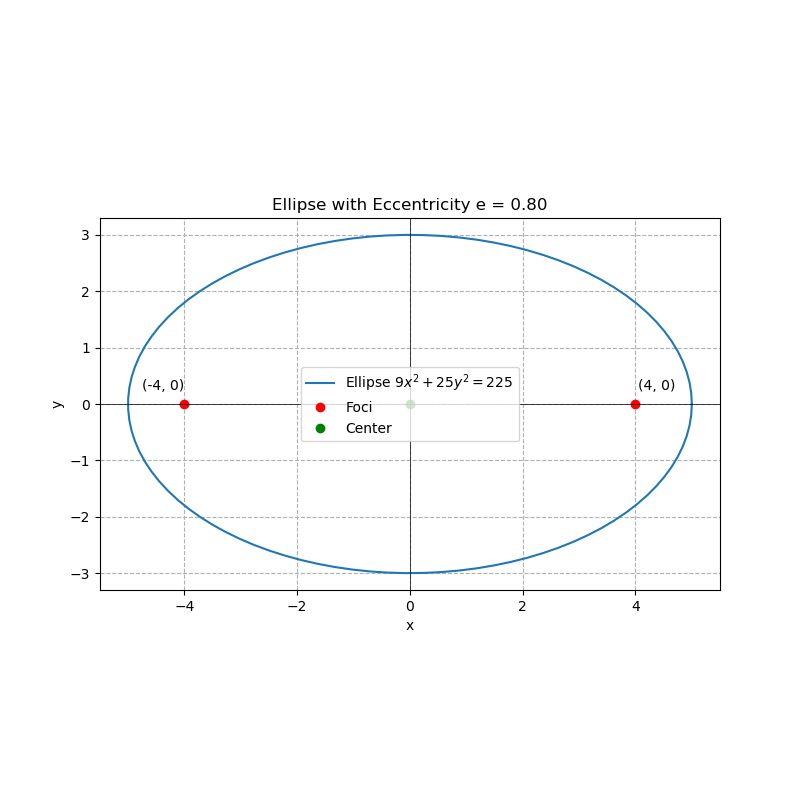
\includegraphics[width=0.8\linewidth]{figs/ellipse.png}
    \caption{}
    \label{fig:placeholder}
\end{figure}



\end{document}






